\documentclass{zirkelblatt}
\usepackage{young}
\geometry{tmargin=2cm,bmargin=3cm,lmargin=3cm,rmargin=3cm}
\usepackage{lscape}
\newcommand{\head}[1]{\section*{\rmfamily #1}}%begin{center}\large \textbf{#1}\end{center}}
\let\raggedsection\centering
\newcommand{\fuzzy}{\mathrel{||}}

%\setkeys{Gin}{draft}
\begin{document}

\maketitle{Klasse 11./12., Gruppe 2}{21. Dezember 2013 \\ und 18. Januar 2014}

\begin{block}{Konventionen}
\begin{itemize}
\item[]
Die \emph{Menge der natürlichen Zahlen} ist~$\NN := \{ 0, 1, 2, 3, \ldots \}$.
\item[]
Die \emph{leere Menge} $\{ \} = \emptyset$ enthält kein einziges Element.
\item[]
Alle Elemente der Menge der Elefanten in diesem Raum können~$\pi$ auswendig.
\end{itemize}
\end{block}

\begin{block}{Regeln für surreale Zahlen}
\renewcommand{\labelenumi}{\arabic{enumi}.}
\begin{enumerate}
\item \emph{Konstruktionsprinzip.}
Sind~$L$ und~$R$ Mengen surrealer Zahlen und \hil{ist kein Element von~$L$
$\geq$ irgendeinem Element von~$R$}, so ist~$\sur{L}{R}$ ebenfalls eine surreale
Zahl. Alle surrealen Zahlen entstehen auf diese Art.

\item \emph{Notation.}
Für~$x = \sur{L}{R}$ bezeichnen wir ein typisches Element von~$L$
mit~"`$x^L$"', ein typisches Element von~$R$ mit~"`$x^R$"'. (Das hat mit
Potenzieren nichts zu tun.) Wenn
wir~"`$\sur{a,b,c,\ldots}{d,e,f,\ldots}$"' schreiben, meinen wir die
Zahl~$\sur{L}{R}$, sodass~$a,b,c,\ldots$ die typischen Elemente von~$L$
und~$d,e,f,\ldots$ die typischen Elemente von~$R$ sind.

\item \emph{Anordnung.}

Wir sagen genau dann~$x \geq y$, falls kein $x^R \leq y$ und~$x \leq$
keinem $y^L$.

Wir sagen genau dann~$x \not\leq y$, wenn~$x \leq y$ nicht gilt.

Wir sagen genau dann~$x < y$, wenn $x \leq y$ und~$y \not\leq x$.

Wir sagen genau dann~$x \leq y$, wenn~$y \geq x$.

Wir sagen genau dann~$x > y$, wenn~$y < x$.

\item \emph{Gleichheit.}
Wir sagen genau dann~$x = y$, wenn~$x \leq y$ und~$y \leq x$.

\item \emph{Rechenoperationen.}
\begin{align*}
  x + y &:= \sur{x^L + y,\ x + y^L}{x^R + y,\ x + y^R}. \\
  -x &:= \sur{-x^R}{-x^L}. \\
  x - y &:= x + (-y). \\
  xy &:= \sur{x^Ly + xy^L - x^Ly^L,\ x^Ry + xy^R - x^Ry^R}{\\&\qquad\qquad\qquad x^Ly + xy^R -
x^Ly^R,\ x^Ry + xy^L - x^Ry^L}.
\end{align*}
\end{enumerate}
\end{block}

\begin{landscape}
\thispagestyle{empty}
\begin{center}
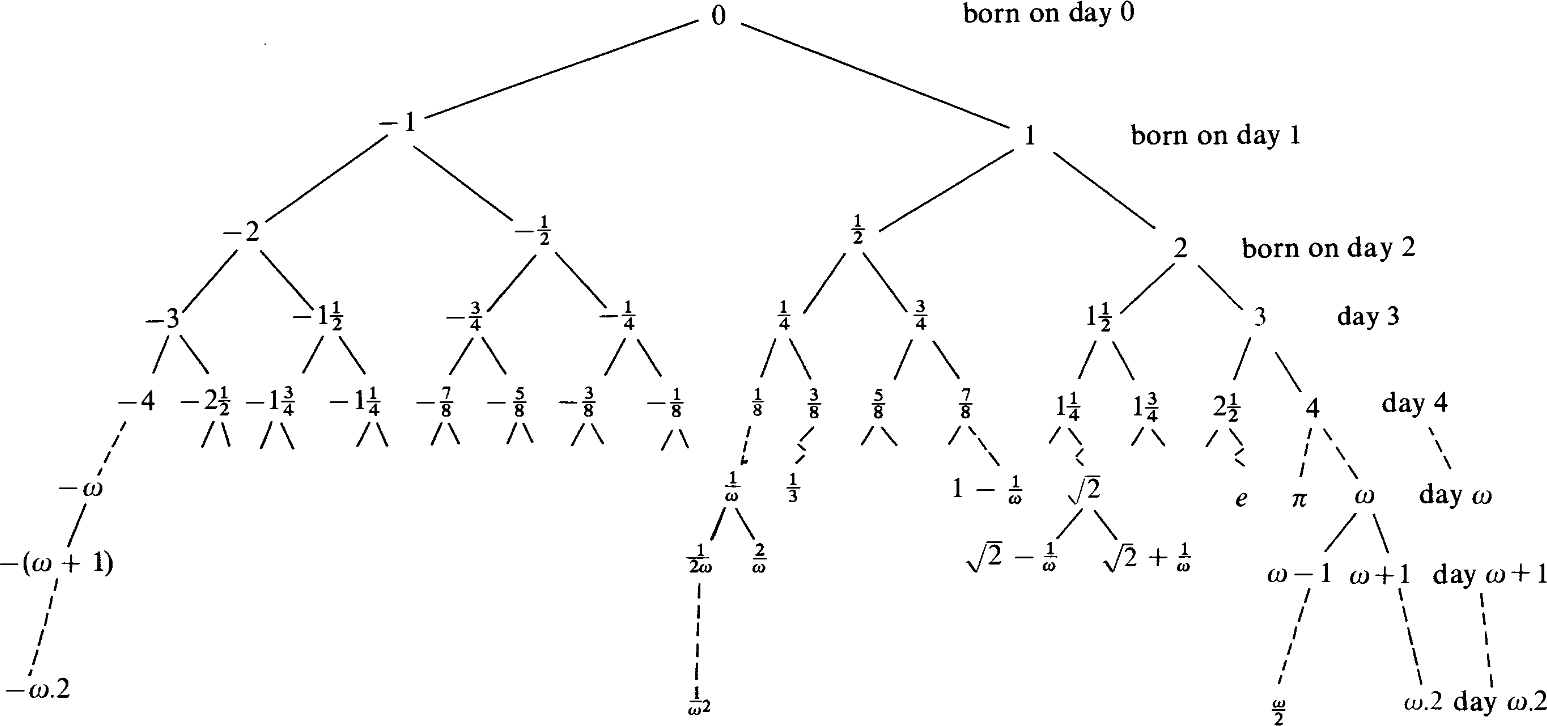
\includegraphics[scale=0.6]{stammbaum-der-surrealen-zahlen}

Abbildung 0 aus Conways Buch: Wann die ersten Zahlen geboren wurden.
\end{center}

\vfill
\textbf{Literatur:}

J. H. Conway. \emph{On Numbers and Games.} Zweite Auflage. A K Peters, 2001. \\
D. Knuth. \emph{Surreal Numbers.} Addison Wesley, 1974. \\
C. Tøndering. \emph{Surreal Numbers.} 2013.
\url{http://www.tondering.dk/claus/sur16.pdf}
\end{landscape}

\addtocounter{aufgabennummer}{-1}

\head{Der kuriose Rechenbereich der surrealen Zahlen}

\begin{aufgabe}{Erste Beispiele für surreale Zahlen}
\label{aufg0}
Zu Beginn ist uns keine einzige surreale Zahl bekannt. Trotzdem kennen wir
eine \emph{Menge} surrealer Zahlen: nämlich die leere Menge. So können wir nach
dem Konstruktionsprinzip eine erste surreale Zahl bauen:
\begin{align*}
  0 &:= \sur{}{} \quad\text{(also $L = R = \emptyset$)} \\
\intertext{Wir haben diese Zahl~"`$0$"' genannt, weil sie die Rolle der Null einnehmen
wird. Mit dieser Zahl an der Hand können wir eine weitere surreale Zahl bauen:}
  1 &:= \sur{0}{} \quad\text{(also $L = \{ 0 \}, R = \emptyset$)}
\end{align*}

\begin{enumerate}
\item Überzeuge dich davon, dass die so definierten Zahlen~$0$ und~$1$ wirklich
surreale Zahlen sind, dass also die \hil{Voraussetzung} in der Konstruktionsvorschrift
jeweils erfüllt war.

\item Überprüfe, dass gemäß der Definitionen tatsächlich~$0 \leq 1$ gilt.

\item Mit der bereits konstruierten Zahl~$0$ kann man insgesamt drei Ausdrücke
angeben:
\[ \sur{0}{}, \quad \sur{}{0}, \quad \sur{0}{0}. \]
Welche der beiden hinteren Ausdrücke sind Zahlen?

\item Sortiere alle bis jetzt gefundenen Zahlen und überlege dir so geeignete
Bezeichnungen für die neuen Zahlen aus~c).

\item Konstruiere ein paar weitere Zahlen, sortiere sie in die bereits
gefundenen Zahlen ein und überlege dir geeignete Namen für sie.
\end{enumerate}
\end{aufgabe}

\begin{aufgabe}{Erste Rechnungen mit surrealen Zahlen (benötigt Aufgabe \ref{aufg0})}
\label{erste-rechnungen}
\begin{enumerate}
\item Überprüfe, dass gemäß der Definitionen gilt: $0 + 0 = 0$.
\item Überprüfe, dass gemäß der Definitionen gilt: $0 + 1 = 1$.
\item Berechne~$(-1) + 1$ und vergleiche das Ergebnis mit~$0$.
\item Erkläre, wieso im Lichte von Teilaufgabe~c) die spezielle
Gleichheitsregel nötig ist: Wieso nennt man zwei surreale Zahlen nicht einfach
genau dann gleich, wenn ihre linken und rechten Mengen übereinstimmen?
\item Berechne~$1 + 1$, berechne~$(1 + 1) + 1$ und so weiter (so lange du
magst). Die Ergebnisse nennen wir fortan~$2$, $3$ und so weiter.
\end{enumerate}
\end{aufgabe}

\begin{aufgabe}{Eine praktische Vereinfachungsregel (benötigt Aufgabe \ref{aufg0})}
\label{vereinfachungsregel}
Es gilt folgendes Lemma: Ohne den Zahlenwert zu verändern, kann man aus der
linken Menge einer surrealen Zahl eine Zahl~$a$ entfernen, sofern es in der
linken Menge noch eine größere Zahl als~$a$ gibt. Analog kann man aus der
rechten Menge einer surrealen Zahl eine Zahl~$b$ entfernen, sofern es in der
rechten Menge noch eine kleinere Zahl als~$b$ gibt.
\begin{enumerate}
\item Überzeuge dich davon, dass folgende Beispielrechnung stimmt:
\[ \sur{0,1,2}{6,7,11} = \sur{0,2}{6} = \sur{2}{6}. \]
\item Vereinfache nach Lust und Laune weitere Zahlen.
\end{enumerate}
\end{aufgabe}

\begin{aufgabe}{Geburtstage von Zahlen (benötigt Aufgabe \ref{aufg0})}
\label{geburtstage}
Der \emph{Geburtstag}~$b(x)$ einer surrealen Zahl ist wiederum eine surreale
Zahl, definiert als
\[ b(x) := \sur{b(x^L), b(x^R)}{}. \]
Wir sagen auch: "`Die Zahl~$x$ wurde am Tag~$b(x)$ geboren."'
\begin{enumerate}
\item Überzeuge dich davon, dass die Zahl~$0$ am Tag~$0$ geboren wurde.
\item Berechne den Geburtstag von einigen surrealen Zahlen.
\item Wieso ergibt die Bezeichnung Sinn? (Vergleiche mit deiner Lösung von
Aufgabe~\ref{aufg0}.)
\item Beweise, dass der Geburtstag einer surrealen Zahl wirklich eine surreale
Zahl ist.
%\item[$\star$ d)] Beweise, dass der Geburtstag einer Zahl stets $\geq 0$ ist.
%(Geht einfacher mit Aufgabe~\ref{zahlenraten}.)
\end{enumerate}
\emph{Bemerkung.} Vielleicht hast du in deiner Bearbeitung von Teilaufgabe~b)
gesehen, dass der Geburtstag zweier verschieden aussehender, aber trotzdem
gleicher surrealen Zahlen nicht unbedingt gleich ist. Das ist ein Manko an obiger
Definition des Geburtstags.
\end{aufgabe}

\begin{aufgabe}{Zahlenwerte erraten (benötigt Aufgabe \ref{geburtstage})}
\label{zahlenraten}
Es gilt folgendes Lemma: Eine Zahl~$x = \sur{x^L}{x^R}$ beschreibt die
\emph{einfachste} -- das heißt \emph{frühest geborene} -- Zahl, die größer als
alle~$x^L$ und kleiner als alle~$x^R$ ist.

\begin{enumerate}
\item Überprüfe, dass dieses Lemma bei den dir bereits bekannten Zahlen stimmt.
\item Errate mit dem Lemma die Werte folgender Zahlen (manche kennst du
vielleicht auch schon):
\[ \sur{1}{}, \qquad
  \sur{2}{}, \qquad
  \sur{-3,1}{2}, \qquad
  \sur{0}{\tfrac{1}{2}}, \qquad
  \sur{-1}{-\tfrac{1}{2},0,\tfrac{1}{2}}. \]
\end{enumerate}
\end{aufgabe}

\begin{aufgabe}{Rechtfertigung einer Bezeichnung (benötigt Aufgabe~\ref{erste-rechnungen})}
Wir definieren~$\tfrac{1}{2} := \sur{0}{1}$. In dieser Aufgabe wollen wir diese
Bezeichnung rechtfertigen.
\begin{enumerate}
\item Berechne~$\tfrac{1}{2} + \tfrac{1}{2}$ gemäß der Definitionen.
\item Beweise, dass das Ergebnis aus Teilaufgabe~a) gleich~$1 = \sur{0}{}$ ist.

\emph{Tipp.} Wenn du Zeit sparen möchtest, kannst du dazu das Lemma aus
Aufgabe~\ref{zahlenraten} verwenden. Streng genommen ist das aber ein
gefährlicher Handel: Denn hier haben wir ja keinen Beweis dieses Lemmas
diskutiert. Deine Rechnung basiert dann daher auf der Annahme, dass ich das
Lemma richtig angegeben habe.
\end{enumerate}

\emph{Bemerkung.} Längere Rechnungen überlässt man lieber dem Computer, als sie
per Hand durchzuführen.
\end{aufgabe}

\begin{aufgabe}{Unendlich große Zahlen (benötigt Aufgabe~\ref{zahlenraten})}
\label{transfinit}
Wir definieren die surreale Zahl
$\omega := \sur{0, 1, 2, \ldots}{}$.
\begin{enumerate}
\item Überzeuge dich davon, dass~$\omega$ wirklich eine surreale Zahl ist.
\item Zeige: Für jede natürliche Zahl~$n$ gilt~$n < \omega$. In diesem Sinn ist
die Zahl~$\omega$ unendlich groß!
\item Berechne $\omega + 1$.
\item Berechne $\omega - 1$.
\item Zeige: Für jede natürliche Zahl~$n$ gilt~$n < \omega - 1$. Die
Zahl~$\omega - 1$ ist also eine Zahl, die immer noch größer als alle
natürlichen Zahlen, aber kleiner als~$\omega$ ist.
\end{enumerate}
\end{aufgabe}

\begin{aufgabe}{Unendlich kleine Zahlen (benötigt Aufgabe~\ref{zahlenraten})}
\label{infinitesimal}
Wir definieren die surreale Zahl
$\varepsilon := \sur{0}{1, \tfrac{1}{2}, \tfrac{1}{4}, \tfrac{1}{8}, \ldots}$.
\begin{enumerate}
\item Überzeuge dich davon, dass~$\varepsilon$ wirklich eine surreale Zahl ist.
\item Beweise: Die Zahl~$\varepsilon$ ist größer als~$0$, aber kleiner als jede
gewöhnliche positive reelle Zahl. Dabei darfst du verwenden, dass jede reelle
Zahl in einem geeigneten Sinn auch als surreale Zahl angesehen werden kann und
dass zu jeder positiven reellen Zahl~$r$ eine Zweierpotenz~$n$
mit~$\tfrac{1}{n} < r$ existiert.
\item Bewundere Ausdrücke wie~$\omega + \varepsilon$, $\omega \cdot
\varepsilon$, $\varepsilon^2, \tfrac{1}{\omega}, \tfrac{1}{\varepsilon}$. Gib
Vermutungen ab, wo sich diese Zahlen auf der
surrealen Zahlengerade einordnen lassen.
\end{enumerate}
\end{aufgabe}

\begin{aufgabe}{Induktionsbeweise mit surrealen Zahlen (benötigt Aufgabe~\ref{aufg0})}
\label{induktionsbeweise}
Wenn man für \emph{alle} surrealen Zahlen~$x = \sur{x^L}{x^R}$ eine bestimmte Aussage
beweisen möchte, kann man dazu so vorgehen: \emph{Unter der Annahme, dass die Aussage für
alle~$x^L$ und alle~$x^R$ schon stimmt, zeigt man, dass sie auch für~$x$
stimmt.} Dieses Beweisprinzip heißt auch \emph{Induktion} und ermöglicht, in
einem Aufwasch eine Behauptung für alle surrealen Zahlen zu beweisen.

Auf den ersten Blick scheint dieses Prinzip zirkulär -- man kann doch nicht das,
was man beweisen möchte, schon voraussetzen! Tatsächlich aber ist dieses
Beweisprinzip durchaus gerechtfertigt. Das wollen wir in dieser Aufgabe verstehen.
\begin{enumerate}
\item Welche besondere Annahme darf man laut Induktionsprinzip treffen, wenn
man den Fall~$x = 0 = \sur{}{}$ beweisen möchte?
\item Im Sinn von Aufgabe~\ref{geburtstage} sind für jede Zahl~$x =
\sur{x^L}{x^R}$ die Zahlen~$x^L$ und~$x^R$
schon \emph{an früheren Tagen} konstruiert worden. Mache dir mit dieser Erkenntnis
und Teilaufgabe~a) klar, dass das Induktionsprinzip zulässig ist.
\item Wenn du das Induktionsprinzip für natürliche Zahlen schon kennst,
wunderst du dich vielleicht, dass man hier nur eine Art Induktionsschritt, aber
keinen Induktionsanfang benötigt. Wieso ist trotzdem alles in Ordnung?
\end{enumerate}
\end{aufgabe}

\begin{aufgabe}{Beispiele für Induktionsbeweise (benötigt
das Prinzip aus Aufgabe~\ref{induktionsbeweise})}
\label{induktionsbeispiele}
\begin{enumerate}
\item Beweise für alle surrealen Zahlen~$x$: $x + 0 = x$.
\item Beweise für alle surrealen Zahlen~$x$: $0 + x = x$.
\item Beweise für alle surrealen Zahlen~$x$: $x \cdot 0 = 0$.
\item Beweise für alle surrealen Zahlen~$x$: $x \geq x$.
\item Beweise für alle surrealen Zahlen~$x$ und~$y$: $x + y = y + x$.
\end{enumerate}
\end{aufgabe}

\begin{aufgabe}{Unmenge surrealer Zahlen (benötigt Aufgabe~\ref{aufg0})}
\label{unmenge}
In einem gewissen Sinn gibt es \emph{zu viele} surreale Zahlen, als dass sie
noch eine Menge bilden könnten; sie bilden nur noch etwas, was man \emph{echte
Klasse} nennt.

Zeige: Wenn die surrealen Zahlen doch eine Menge bilden würden, gäbe es eine
surreale Zahl, die größer als alle surrealen Zahlen wäre, insbesondere also auch
größer als sich selbst.
\end{aufgabe}
%\begin{loesung}
%Angenommen, die surrealen Zahlen bilden eine Menge. Dann können wir eine surreale
%Zahl~$\Omega$ mit~$L := \text{Menge aller surrealen Zahlen}$ und~$R :=
%\emptyset$ bilden. Denn da~$R$ keine Elemente enthält, ist die
%\hil{Voraussetzung} in der Konstruktionsvorschrift erfüllt. Durch Induktion
%können wir zeigen, dass~$\Omega > x$ für alle surrealen Zahlen~$x$.
%\end{loesung}

\begin{aufgabe}{Ordinale Addition (benötigt Aufgabe~\ref{zahlenraten})}
\label{ordinale-addition}
In dieser Aufgabe wollen wir eine Rechenoperation
kennenlernen, die beim Spiel \emph{Hackenbush} eine Rolle spielen wird (siehe
Aufgabe~\ref{game-hackenbush}). Die \emph{ordinale Summe} der surrealen Zahl~$1$ mit
einer weiteren surrealen Zahl~$x$ ist definiert als
\[ 1 \boxplus x := \sur{0,\ 1 \boxplus x^L}{1 \boxplus x^R}. \]
Wie die ordinale Summe von zwei beliebigen Summanden definiert ist,
diskutieren wir hier nicht.
\begin{enumerate}
\item Überzeuge dich von folgenden Rechnungen:
\[ 1 \boxplus 0 = 1, \quad
  1 \boxplus 1 = 2, \quad
  1 \boxplus 2 = 3. \]
\item Was ist~$1 \boxplus (-1)$?
\item Was ist~$1 \boxplus \tfrac{1}{2}$?
\item Zeige: Für jede Zahl~$x$ ist~$1 \boxplus x$ positiv (d.\,h. $> 0$).
\item Man kann beweisen, dass sich für eine surreale Zahl~$x$, die eine gewöhnliche
reelle Zahl repräsentiert, der Wert der ordinalen Summe~$1 \boxplus x$ wie
folgt ergibt: Er ist der erste Bruch in der Folge
\[ \frac{x+1}{1}, \quad
  \frac{x+2}{2}, \quad
  \frac{x+3}{4}, \quad
  \frac{x+4}{8}, \quad
  \frac{x+5}{16}, \quad \ldots, \]
dessen Zähler (so, wie er geschrieben steht) größer als oder gleich~$1$ ist. Verwende diese
Regel, um die Rechnungen aus den ersten drei Teilaufgaben schnell und einfach
zu wiederholen, und berechne nach Lust und Laune weitere ordinale Summen.
\end{enumerate}
\end{aufgabe}


\head{Kombinatorische Spiele}

\begin{center}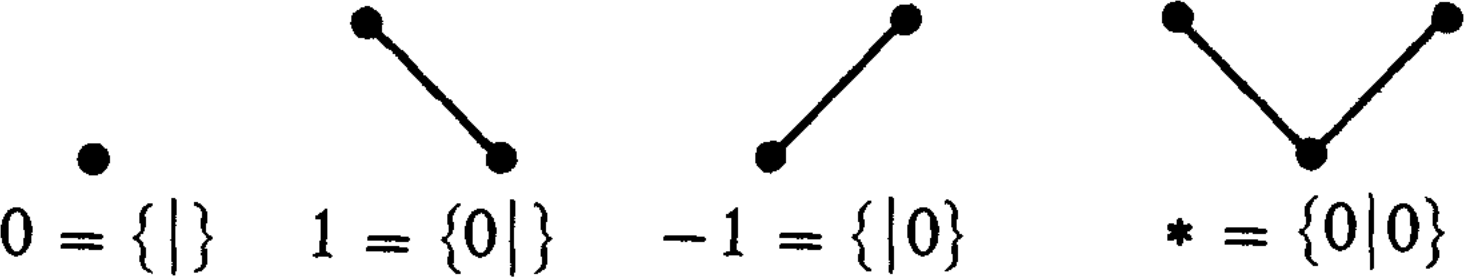
\includegraphics[scale=0.2]{einfache-spiele}\end{center}

In diesem Abschnitt wollen wir rundenbasierte Zwei-Personen-Spiele betrachten,
die von einem \emph{linken} und einem \emph{rechten Spieler} bestritten werden,
keinerlei Zufallselemente enthalten und nicht mit verborgenen Informationen
arbeiten: Alle möglichen Züge sind für beide Spieler erkennbar. Verlierer ist
derjenige, der keinen Zug mehr tätigen kann. Das Mühlespiel ist etwa ein
solches Spiel, Fußball und viele Kartenspiele nicht.

Die jeweils vorliegenden Spielsituationen, genannt \emph{Positionen}, wollen wir
mathematisch mit sog. \emph{Games} beschreiben, einer leichten
Verallgemeinerung der surrealen Zahlen. Die Konstruktionsregel der Games ist
im Vergleich zur surrealen Variante freigiebiger:

\emph{Konstruktionsregel für Games.}
Sind~$L$ und~$R$ Mengen von Games,
so ist~$\sur{L}{R}$ ebenfalls ein Game. Alle Games entstehen auf diese Art.

Die restlichen Regeln für Games sind dieselben wie für die surrealen Zahlen,
und das Induktionsprinzip (siehe Aufgabe~\ref{induktionsbeweise}) gilt
ebenfalls.

Die linke Menge eines Games stellen wir uns als die Menge derjenigen Positionen
vor, in die der linke Spieler ziehen darf, wenn er am Zug ist. Analog
beschreibt die rechte Menge eines Games diejenigen Positionen, in die der rechte
Spieler ziehen darf, wenn er am Zug ist. Fortan wollen wir den linken Spieler
auch einfach \emph{Links} und den rechten \emph{Rechts} nennen.

Das einfachste Zwei-Personen-Spiel ist das sog. \emph{Nullspiel}: Der Spieler,
der an der Reihe ist, verliert sofort. In diesem Spiel haben also beide Spieler
keine erlaubten Züge -- die Menge ihrer erlaubten Züge sind also jeweils leer.
Diese Situation wird daher durch das Game~$\sur{}{} = 0$ beschrieben.

Die zweite Abbildung oben zeigt eine Spielsituation, in dem (ausgehend vom Wurzelknoten
unten) Links einen erlaubten Zug durchführen kann. Das soll die
nach links geneigte Kante andeuten. Rechts hat keinerlei erlaubte
Züge. Daher ist die rechte Menge des zugehörigen Games leer. Die linke Menge
enthält genau ein Element, nämlich das Game, das die Spielsituation nach
Tätigung des einzigen erlaubten Zugs beschreibt. Da diese das Nullspiel ist,
gilt also~$L = \{ 0 \}$. Somit beschreibt das Game~$\sur{0}{} = 1$ die
Spielsituation.

Dual dazu beschreibt das Game~$\sur{}{0} = -1$ eine Spielsituation, in dem
Links keinerlei erlaubte Züge hat (also sofort verliert, wenn er oder sie an der
Reihe ist) und Rechts mit einem Zug in das Nullspiel ziehen darf, in dem
dann Links verliert, da Links keinen Zug mehr tätigen kann.

Die Games~$0$, $1$ und~$-1$ sind sogar surreale Zahlen. Das Game, das die
Spielsituation der vierten Abbildung oben beschreibt, ist daher unser erstes
Beispiel für ein Game, das keine surreale Zahl ist. Beide Spieler haben genau
einen erlaubten Zug, der jeweils zum Nullspiel führt. Als Kurzschreibweise
definieren wir~$\star := \sur{0}{0}$.

Jede surreale Zahl ist entweder~$> 0$, $= 0$ oder~$< 0$. Bei Games kann es
vorkommen, dass keine dieser Möglichkeiten eintritt. Wir sagen dann, das Game
sei \emph{unklar} und schreiben~"`$\fuzzy 0$"'. Allgemein gilt für ein Game~$G$:

\begin{center}\framebox{\begin{minipage}{0.9\textwidth}\vspace{-1.3em}
\begin{align*}
  G > 0 &\text{ genau dann, wenn es eine Gewinnstrategie für Links gibt.} \\
  G < 0 &\text{ genau dann, wenn es eine Gewinnstrategie für Rechts gibt.} \\
  G = 0 &\text{ genau dann, wenn es eine Gewinnstrategie für den zweiten Spieler gibt.} \\
  G \fuzzy 0 &\text{ genau dann, wenn es eine Gewinnstrategie für den ersten Spieler gibt.}
\end{align*}\end{minipage}}\end{center}
Der Ausdruck \emph{Gewinnstrategie} bedeutet, dass der betreffende Spieler in
der Lage ist, einen Sieg zu erzwingen -- unabhängig davon, wie sein Gegenüber
reagiert. Dabei ist aber nicht ausgeschlossen, dass der betreffende Spieler aus
Unachtsamkeit einen Fehler macht und daher trotzdem verliert.

\vspace{1em}


\begin{aufgabe}{Gewinnstrategien bei den vier einfachsten Spielen (benötigt
Aufgabe~\ref{aufg0})}
\label{analyse4}
Mache dir ohne Verwendung der Merkregeln im Kasten klar:
\begin{enumerate}
\item Im Spiel~$1$ gibt es eine Gewinnstrategie für Links -- unabhängig davon,
welcher Spieler beginnt.
\item Im Spiel~$-1$ gibt es eine Gewinnstrategie für Rechts -- unabhängig davon,
welcher Spieler beginnt.
\item Im Spiel~$\star$ gibt es eine Gewinnstrategie für den beginnenden Spieler,
wer immer das auch sein mag.
\item Im Spiel~$0$ gibt es eine Gewinnstrategie für den zweiten Spieler.
\end{enumerate}
\end{aufgabe}

\begin{aufgabe}{Gewöhnung an unklare Games (benötigt Aufgabe~\ref{analyse4})}
Beweise rechnerisch, dass~$\star \fuzzy 0$, beweise also, dass weder~$\star
\leq 0$ noch~$\star \geq 0$ stimmt.
\end{aufgabe}

\begin{aufgabe}{Gewinnstrategien bei allgemeinen Games (benötigt
Aufgabe~\ref{analyse4} und viel Ruhe)}
\label{gewinnstrategien}
In dieser Aufgabe wollen wir verstehen, wieso für Games~$G$ aus~$> 0$, $<
0$, $= 0$ bzw. $\fuzzy 0$ schon folgt, dass es eine Gewinnstrategie für Links,
Rechts, den zweiten Spieler bzw. den ersten Spieler gibt. Dazu wollen wir diese
Aussage über Induktion beweisen; sei also ein Game~$G = \sur{G^L}{G^R}$
gegeben und gelte die zu zeigende Behauptung schon für alle Games~$G^L$
und~$G^R$.
\begin{enumerate}
\item Überzeuge dich von folgenden Beziehungen:
\begin{align*}
  G > 0 &\text{ genau dann, wenn $\text{kein $G^R$} \leq 0$ und~$0 \leq \text{einem $G^L$}$.} \\
  G < 0 &\text{ genau dann, wenn $0 \leq \text{keinem $G^L$}$ und~$\text{ein $G^R$} \leq 0$.} \\
  G = 0 &\text{ genau dann, wenn $0 \leq \text{keinem $G^L$}$ und~$\text{kein $G^R$} \leq 0$.} \\
  G \fuzzy 0 &\text{ sonst.}
\end{align*}
\item Nun wollen wir in jedem der vier Fälle zeigen, dass tatsächlich eine Gewinnstrategie
wie behauptet existiert. Vervollständige folgenden Beweisansatz für den Fall~$G
> 0$:

\emph{Falls~$G > 0$: Dann ist zu zeigen, dass Links eine
Gewinnstrategie besitzt. Falls Links beginnt, so kann er in eine Position~$G^L
\geq 0$ ziehen. Diese neue Position ist also $> 0$ oder~$= 0$. Im ersten Fall
hat er nach Induktionsvoraussetzung eine Gewinnstrategie. Im zweiten Fall hat
nach Induktionsvoraussetzung der zweite Spieler eine Gewinnstrategie -- dieser
ist auch gerade Links. Falls Rechts beginnt, so \ldots}
\item Führe auf ähnliche Art und Weise Beweise in den drei restlichen Fällen.
Der Fall~$G \fuzzy 0$ ist der schwerste.
\end{enumerate}
\end{aufgabe}

\begin{aufgabe}{Interpretation der Negation (benötigt Aufgabe~\ref{analyse4})}
\label{game-negation}
\begin{enumerate}
\item Mache dir klar: Wird eine Spielsituation durch ein Game~$G =
\sur{G^L}{G^R}$ beschrieben,
so beschreibt~$-G = \sur{-G^R}{-G^L}$ dieselbe Spielsituation, wobei aber die Rollen des linken und
rechten Spielers für den ersten und alle weiteren Züge genau vertauscht sind.
\item Erkläre, wieso die Negation
eines unklaren Games wieder ein unklares Game ist.
\end{enumerate}
\end{aufgabe}

\begin{aufgabe}{Interpretation der Addition (benötigt Aufgabe~\ref{analyse4})}
\label{game-addition}
\begin{enumerate}
\item Mache dir klar: Werden zwei Spielsituationen durch Games~$G =
\sur{G^L}{G^R}$ und~$H = \sur{H^L}{H^R}$ beschrieben, so beschreibt die Summe~$G
+ H = \sur{G^L + H,\ G + H^L}{G^R + H,\ G + H^R}$ folgende Situation: Die
Spiele zu~$G$ und~$H$ liegen auf dem Tisch. Der beginnende Spieler darf sich
nach Belieben eines der beiden Spiele aussuchen und dort einen für ihn
erlaubten Zug tätigen. Danach darf der zweite Spieler im gleichen oder im
anderen Spiel einen Zug tätigen. Auf diese Weise machen die beiden Spieler so
lange weiter, bis einer der Spieler in keinem der beiden Einzelspiele einen Zug
tätigen kann; dann hat dieser verloren.
\item Illustriere das Game~$1 + 1$.
\item Illustriere das Game~$1 + (-1)$ und mache dir klar, dass es
spieltechnisch gleich dem Nullspiel ist.
\item Illustriere das Game~$\star + \star$ und mache dir klar, dass auch dieses
Game spieltechnisch gleich dem Nullspiel ist.
\end{enumerate}
\end{aufgabe}

\begin{aufgabe}{Interpretation von~$G - G$ (benötigt
Aufgaben~\ref{game-negation} und~\ref{game-addition})}
\label{game-gg}
\begin{enumerate}
\item Erkläre, wie man als Schachlaie gegen einen von zwei Großmeistern
gewinnen kann, wenn man mit den beiden Großmeistern gleichzeitig spielen darf.
\item Beweise, dass für jedes Game~$G$ das Game~$G - G = G + (-G)$ spieltechnisch
gleich dem Nullspiel ist, dass also der zweite Spieler eine Gewinnstrategie
besitzt.
\end{enumerate}
\end{aufgabe}

\begin{aufgabe}{Ein Spiel mit Dominosteinen (benötigt Aufgabe~\ref{game-addition})}
\label{game-domino}
Auf einem gleichmäßig in Quadrate eingeteilten Spielbrett platzieren linker und
rechter Spieler abwechselnd Dominosteine. Ein solcher überdeckt immer genau
zwei Quadrate. Der linke Spieler darf seine Steine nur vertikal, der rechte
Spieler nur horizontal legen; die Steine dürfen nicht überlappen. Verloren hat,
wer keinen Zug mehr tätigen kann.
\begin{enumerate}
\item Überzeuge dich davon, dass wenn nur noch ein Kästchen frei ist, der als
nächstes ziehende Spieler verliert. Diese Spielposition wird also durch das
Game~$0$ beschrieben.
\[
  \begin{Young}
    \cr
  \end{Young}
\]
\item In welche Positionen können die beiden Spieler ziehen, wenn nur noch drei Kästchen in
einer vertikalen Reihe frei ist? Überzeuge dich davon, dass diese Situation
durch das Game~$1 = \sur{0}{}$ beschrieben wird.
\[
  \begin{Young}
    \cr
    \cr
    \cr
  \end{Young}
\]
\item Bewerte folgende Spielsituationen mit Games (dargestellt ist jeweils der
noch freie Bereich). \emph{Zur Kontrolle:} Es
kommen die Games~$-2, -1, \tfrac{1}{2}, 1, \star, \sur{1}{-1}$ vor.
\[
  \begin{Young}
    &\cr
  \end{Young}
  \quad\qquad
  \begin{Young}
    \cr
    \cr
    \cr
  \end{Young}
  \quad\qquad
  \begin{Young}
    &&&\cr
  \end{Young}
  \quad\qquad
  \begin{Young}
    \cr
    \cr
    &\cr
  \end{Young}
  \quad\qquad
  \begin{Young}
    \cr
    &\cr
  \end{Young}
  \quad\qquad
  \begin{Young}
    &\cr
    &\cr
  \end{Young}
\]
\item Wenn der noch freie Bereich in voneinander getrennte Teilbereiche
zerfällt, ist das Game, das die Situation beschreibt, gleich der Summe der
Games zu den Teilbereichen. Nutze diese Beobachtung, um nur unter Verwendung
von Teilaufgabe~c) sofort das Game zu folgender Situation anzugeben. Welcher
Spieler besitzt eine Gewinnstrategie?
\[
  \begin{Young}
    \cr
    \cr
    &\cr
  \end{Young}
  \begin{array}{@{}c@{}}\begin{Young}
    &&&\cr
  \end{Young}\\[7.2em]\end{array}
  \hspace{-3.7em}
  \begin{Young}
    \cr
    \cr
  \end{Young}
\]
\vspace{-5em}
\item Zeichne nach Lust und Laune weitere Spielsituationen und bestimme ihre
Bewertungen durch Games.
\item Sind nur noch vier horizontal zusammenhängende Kästchen frei, gewinnt der
rechte Spieler. Das stimmt auch bei nur noch zwei horizontal zusammenhängenden
Kästchen, lax gesprochen ist da der Vorsprung aber "`knapper"'. Wie drückt
sich das in der Bewertung durch Games aus?
\item Hast du eine Idee, inwieweit der linke Spieler in der Situation aus Teilaufgabe~c) mit
Bewertung~$\tfrac{1}{2}$ tatsächlich \emph{einen halben Zug Vorsprung}
gegenüber dem rechten Spieler hat?
\item Sei eine Spielsituation des Dominospiels durch ein Game~$G =
\sur{G^L}{G^R}$ beschrieben.
Welche Situation beschreibt dann das negierte Game~$-G = \sur{-G^R}{-G^L}$?
(Benötigt Aufgabe~\ref{game-negation}.)
\end{enumerate}
\end{aufgabe}

\begin{aufgabe}{Hackenbush (benötigt Aufgabe~\ref{analyse4})}
\label{game-hackenbush}
Das Spiel \emph{Hackenbush} wird nicht auf einem regelmäßigen Schachbrett oder
einem Käst\-chen\-pa\-pier gespielt, sondern auf einem beliebigen \emph{Graphen}.
Conway gibt etwa folgendes Beispiel:
\begin{center}
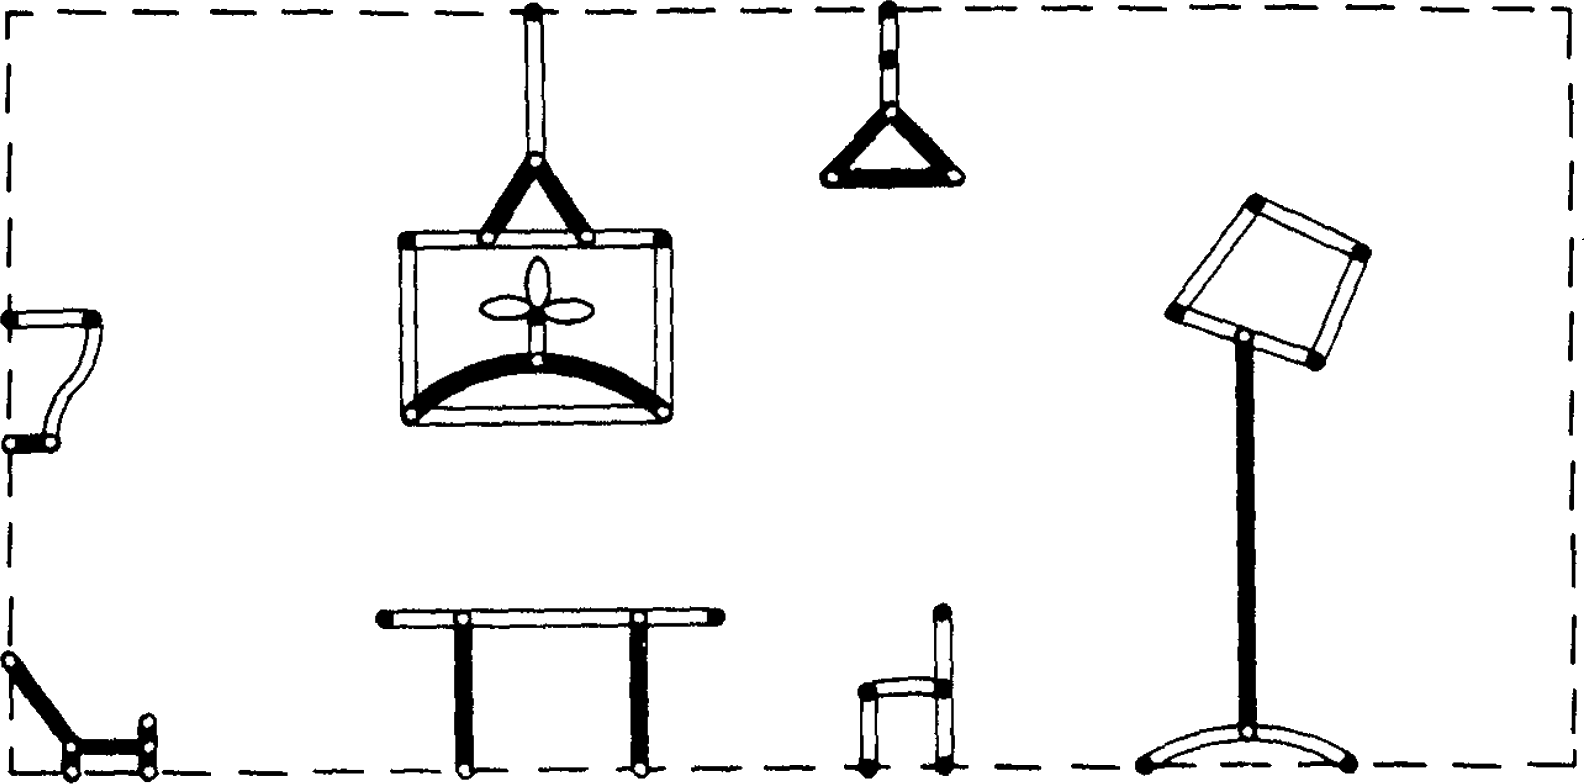
\includegraphics[scale=0.2]{hackenbush}
\end{center}
Dabei sind gewisse \emph{Knoten} (Pünktchen) mittels schwarzer und weißer
\emph{Kanten} (gerade oder krumme Linien) verbunden. Die gestrichelte Umrandung
heißt \emph{Grund}, und jeder Knoten muss über eine Folge (beliebig gefärbter)
Kanten mit dem Grund verbunden sein. Der linke Spieler darf in
jedem Zug nach Belieben eine schwarze Kante, der rechte Spieler eine weiße
Kante hacken und damit aus dem Spiel entfernen. Alle Knoten und Kanten, die
danach nicht mehr mit dem Grund verbunden sind, werden ebenfalls entfernt.
Verloren hat, wer keinen Zug mehr tätigen kann.
\begin{enumerate}
\item Überzeuge dich von folgenden Bewertungen durch Games:
\begin{center}
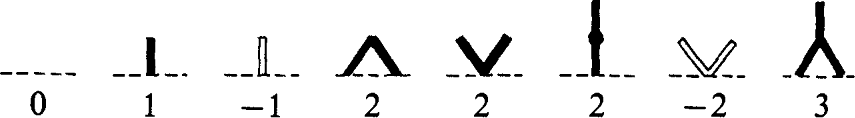
\includegraphics[scale=0.4]{hackenbush-beispiele-1}
\end{center}
\item Welchen Wert haben die folgenden Situationen?
\begin{center}
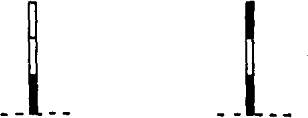
\includegraphics[scale=0.6]{hackenbush-beispiele-2}
\end{center}
% Bei Nummerierungsänderung auch weiter unten in dieser Aufgabe anpassen.
\item Sei eine Spielsituation von Hackenbush durch ein Game~$G =
\sur{G^L}{G^R}$ beschrieben.
Welche Situation beschreibt dann das negierte Game~$-G = \sur{-G^R}{-G^L}$?
(Benötigt Aufgabe~\ref{game-negation}.)
\item Es ist keine einfache Regel bekannt, mit der man den Wert eines
beliebigen Graphen bestimmen könnte. Für Graphen, die sogar \emph{Bäume} sind,
d.\,h. keine \emph{Schleifen} enthalten, können wir aber eine einfache Regel
angeben. Grundlegend dafür ist folgende Beobachtung: Kennen wir schon den
Wert~$G$ eines Teilstücks~$P$, so ist der Wert
der zusammengesetzten Situation
\begin{center}

\includegraphics[scale=0.3]{hackenbush-beispiele-3}
\end{center}
gleich~$1 \boxplus G$ (siehe Aufgabe~\ref{ordinale-addition} für diese
Rechenoperation). Beweise diesen Sachverhalt!
\item Wie errechnet sich der Wert, wenn analog zur vorherigen Teilaufgabe
zu einem Teilstück~$P$ eine \emph{weiße} Kante hinzugefügt ist? \emph{Tipp:}
Verwende zweimal Teilaufgabe~c).
\item Verwende die Erkenntnisse aus der vorherigen beiden Teilaufgaben, um von
mehren Bäumen deiner Wahl das zugehörige Game zu berechnen.
\end{enumerate}
\end{aufgabe}

\begin{aufgabe}{Hackenbush auf unendlichen Graphen (benötigt
Aufgabe~\ref{game-hackenbush})}
\label{game-hackenbush-infinite}
\begin{enumerate}
\item Auf manchen unendlichen Graphen kann man ebenfalls Hackenbush spielen.
Welchen Wert hat der Graph, der neben einer Umrandung unten nur aus einem
linienförmigen Wolkenkratzer mit unendlich vielen Stockwerken, der aus
unendlich vielen schwarzen Kanten zusammengesetzt ist, besteht? Welchen Wert
hat die Situation, wenn man eine einzelne direkt mit dem Grund verbundene weiße
Kante hinzufügt? Diese Aufgabe benötigt Aufgabe~\ref{transfinit}.
\item Wieso kann man \emph{nicht} auf einem Graphen spielen, der unendlich
viele nebeneinander platzierte Kopien des Wolkenkratzers aus der vorherigen
Teilaufgabe enthält?
\end{enumerate}
\end{aufgabe}

%\begin{aufgabe}{Meine Mutter verdient mehr als deine (benötigt
%Aufgabe~\ref{analyse4})}
%Linker und rechter Spieler wollen damit angeben, dass ihre Mutter mehr Geld als
%die jeweils andere Mutter verdient. Dazu nennt einer der beiden Spieler eine
%Zahl, die angeblich das Gehalt seiner Mutter angibt. Daraufhin nennt der zweite
%Spieler eine Zahl, die genauso fiktiv das Gehalt seiner Mutter angeben soll.
%Damit endet das Spiel; gewonnen hat der, der die größere Zahl gesagt hat.
%
%Mache dir klar, dass dieses Spiel durch
%\end{aufgabe}


\head{Nimbers}

\begin{aufgabe}{Mex-Operation}
\label{mex}
Ist~$S$ eine endliche Menge natürlicher Zahlen, so ist~$\mex S$ die \emph{kleinste}
natürliche Zahl, die \emph{nicht} in~$S$ liegt (minimum excludant).
\begin{enumerate}
\item Überzeuge dich von der Richtigkeit folgender Beispiele:
\[
  \mex \{ 0,1,4,7 \} = 2, \quad
  \mex \{ 1,4,7 \} = 0, \quad
  \mex \emptyset = 0. \]
\item Berechne das Mex von deiner Lieblingsteilmenge natürlicher Zahlen.
\end{enumerate}
\end{aufgabe}

\begin{aufgabe}{Nimber-Addition (benötigt Aufgabe \ref{mex})}
\label{nimber-addition}
Die \emph{Nimber-Addition} ist in mengentheoretischer Notation wie folgt rekursiv definiert:
\[ n \oplus m := \mex\Bigl(\left\{n' \oplus m \,|\, n' < n\right\} \cup
\left\{n \oplus m' \,|\, m' < m\right\}\Bigr). \]
Wenn man also den Wert von~$n \oplus m$ herausfinden möchte, muss man zunächst
die Werte von~$n' \oplus m$ für alle kleineren Zahlen~$n' < n$ und die Werte
von~$n \oplus m'$ für alle kleineren Zahlen~$m' < m$ bestimmen. Der Wert
von~$n \oplus m$ ergibt sich dann als Mex dieser Zahlen. \emph{Achtung,} die
Schreibweise hier ist verwirrend. Die senkrechten Striche in der Definition
von~$n \oplus m$ haben nichts mit der Abgrenzung zwischen linker und rechter
Menge bei surrealen Zahlen zu tun.
\begin{enumerate}
\item Ergänze unten stehende Tabelle für die Nim-Addition.
\item[$\star$ b)] Wenn du die Beweistechnik der Induktion für natürliche Zahlen kennst, kannst
du beweisen, dass für alle~$n \in \NN$ gilt: $0 \oplus n = n$.
% n \oplus n &= 0
\end{enumerate}
\begin{center}
  \begin{tabular}{r|ccccccccl}
    $n \setminus m$ & 0 & 1 & 2 & 3 & 4 & 5 & 6 & 7 & $\cdots$ \\\hline
    0 & 0 & 1 & 2 \\
    1 &   & 0 & 3 \\
    2 & \\
    3 & & & & & & & 4 \\
    4 & & & 6 \\
    5 & \\
    6 & \\
    7 & & & & & & 2 \\
    \vdots
  \end{tabular}
\end{center}
\end{aufgabe}

\begin{aufgabe}{Interpretation der Nimber-Addition im Binärsystem
(benötigt Aufgabe~\ref{nimber-addition})}
\label{nimber-addition-binaer}
Im gewöhnlichen Zehnersystem gibt es die Ziffern von~$0$ bis~$9$. Der Wert
einer Ziffer ergibt sich von rechts nach links über die Zehnerpotenzen: Einer,
Zehner, Hunderter, Tausender, usw. Das Binärsystem ist viel einfacher: Da gibt
es nur die Ziffern~$0$ und~$1$. Der Wert einer Ziffer ergibt sich dann von
rechts nach links über die Zweierpotenzen: Einer, Zweier, Vierer, Achter,
Sechzehner, usw. Schreibt man eine Zahl im Binärsystem, so macht man das durch
einen nachgestellten Index deutlich.
\begin{enumerate}
\item Überzeuge dich von der Richtigkeit folgender Beispiele:
\[ 3 = 11_2, \qquad
  6 = 110_2, \qquad
  10 = 1010_2, \qquad
  16 = 10000_2. \]
\item Überlege dir, wie man im Binärsystem schriftlich addieren kann, und
rechne einige Beispiele.
\item Die Nimber-Addition funktioniert nun genau wie die schriftliche
Binäraddition, nur dass man \emph{alle Überträge ignoriert}. Rechne mit dieser
Einsicht so viele Einträge der Tabelle aus Aufgabe~\ref{nimber-addition} nach,
wie du magst.
\end{enumerate}
\end{aufgabe}

\begin{aufgabe}{Das Nim-Spiel (benötigt Aufgabe~\ref{game-addition})}
\label{nim}
Bei Nim spielt man mit mehreren Haufen von gleichartigen Spielsteinen. Die
erlaubten Züge sind für beide Spieler dieselben: Wenn man an der Reihe ist,
darf man sich nach Belieben einen der Haufen aussuchen und muss dann in diesem eine
beliebige Anzahl von Spielsteinen, mindestens jedoch einen, entfernen. Verloren
hat, wer keinen Zug mehr tätigen kann. Spiele, bei denen beide Spieler stets
dieselben Zugmöglichkeiten haben, heißen auch \emph{neutrale Spiele} (engl.
\emph{impartial games}).
\begin{enumerate}
\item Überzeuge dich davon, dass der Fall nur eines Haufens, der auch nur aus
einem Spielstein besteht, durch das Game~$\star = \sur{0}{0}$ beschrieben wird.
Welcher Spieler besitzt eine Gewinnstrategie?
\item Überzeuge dich davon, dass der Fall nur eines Haufens, der aus genau zwei
Spielsteinen besteht, durch das Game~$\sur{0,\star}{0,\star}$ beschrieben
werden kann.
\item Wie drückt sich in den Games aus, dass die beiden Spieler dieselben
Zugmöglichkeiten haben?
\item Seien zwei Haufen gegeben, wobei der eine durch ein Game~$G$ und der
andere durch ein Game~$H$ beschrieben wird. Wodurch wird dann die
zusammengesetzte Spielsituation beschrieben?
\end{enumerate}
Das Nim-Spiel ist für die Theorie sehr wichtig. Es ist nämlich nicht nur das
Paradebeispiel für ein neutrales Spiel, sondern gewissermaßen das
\emph{universelle} neutrale Spiel: Jede Spielsituation eines \emph{jeden}
neutralen Spiels ist äquivalent zu einer Position des Nim-Spiels. Diese
tiefgehende Beobachtung wollen wir in Aufgabe~\ref{sprague-grundy} verstehen.
\end{aufgabe}

\begin{aufgabe}{Nimbers (benötigt Aufgabe~\ref{nim})}
\label{nimbers}
Für jede natürliche Zahl~$n$ definieren wir das Game
\[ \star n := \sur{L}{R}, \quad
\text{wobei~$L = R = \{ \star 0, \star 1, \ldots, \star(n-1) \}$.} \]
Linke und rechte Menge von~$\star n$ sind also identisch, und zwar enthalten
sie beide die Games~$\star n'$ für~$0 \leq n' < n$. Games der Form~$\star n$
heißen \emph{Nimbers}.
\begin{enumerate}
\item Überzeuge dich von der Richtigkeit folgender Beispiele:
\[ \star 0 = 0, \quad
  \star 1 = \star, \quad
  \star 2 = \sur{0,\star}{0,\star}. \]
\item Sei beim Nim-Spiel nur ein Haufen gegeben, wobei dieser aus~$n$
Spielsteinen bestehe. Durch welches Game wird diese Spielsituation beschrieben?
Kannst du deine Vermutung beweisen?
% Falls sich die Nummerierung der folgenden Teilaufgabe ändert,
% auch bei zusammenhang-mex anpassen.
\item Begründe, dass für alle natürlichen Zahlen~$n$ die Rechenregel
$\star n = -(\star n)$
gilt. Das kannst du entweder spieltheoretisch machen (beachte dazu
Aufgabe~\ref{game-negation}) oder durch einen Induktionsbeweis über~$n$.
% Falls sich die Nummerierung der folgenden Teilaufgabe ändert,
% auch bei zusammenhang-mex anpassen.
\item Welche Spielsituation beschreibt das Game~$\star n + \star n$, wobei~$n$
eine natürliche Zahl ist? Begründe, dass diese Situation äquivalent zum
Nullspiel ist, dass also der zweite Spieler stets gewinnen kann. In Formeln
kann man diese Beobachtung so festhalten: $\star n + \star n = 0.$
\item Zeige für alle natürlichen Zahlen~$n \geq 1$: $\star n \fuzzy 0$.
\end{enumerate}
\end{aufgabe}

\begin{aufgabe}{Zusammenhang zur Mex-Operation (benötigt Aufgaben~\ref{mex}
und~\ref{nimbers} und viel Ruhe)}
\label{zusammenhang-mex}
Sei~$S = \{ s_1,\ldots,s_m \}$ eine endliche Menge natürlicher Zahlen und~$\mex
S$ ihr Meximum. In dieser Aufgabe wollen wir verstehen, wieso die Beziehung
\[ \sur{\star s_1,\ldots,\star s_m}{\star s_1,\ldots,\star s_m} + \star(\mex S)
= 0
\]
gilt. Diese Vereinfachungsregel werden wir nutzen, um den Zusammenhang zur
Nimber-Addition zu klären.
\begin{enumerate}
\item Erkläre, welche Spielsituation durch das Game auf der linken Seite der
Gleichung beschrieben wird. In welche Positionen kann der beginnende Spieler
ziehen? Beachte, dass sich die Situation aus zwei Teilspielen (dem zum vorderen
und dem zum hinteren Summanden) zusammensetzt.
\begin{center}
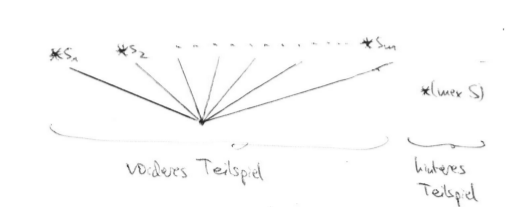
\includegraphics[scale=0.6]{rechenregel-mex}
\end{center}
\item Zeige nun, dass diese Spielsituation äquivalent zum Nullspiel ist, dass
also der beginnende Spieler verliert. Damit ist dann die Rechenregel bewiesen.
Vervollständige dazu folgenden Beweisansatz:

\emph{Fall 1: Der beginnende Spieler tätigt einen Zug im vorderen Teilspiel: Er
zieht dort in die Situation~$\star s_i$. Danach liegen also zwei Teilspiele
vor: Zum einen~$\star s_i$, zum anderen immer noch~$\star(\mex S)$. Nun
kann~$\mex S$ größer oder kleiner als~$s_i$ sein, aber nicht gleich (wieso?).
Falls es größer ist, kann der zweite Spieler im hinteren Teilspiel in die
Situation~$\star s_i$ ziehen (wieso?). Danach liegen also zwei Teilspiele vor:
Zum einen~$\star s_i$, zum anderen jetzt ebenfalls~$\star s_i$. Nach
Teilaufgabe~d) von Aufgabe~\ref{nimbers} kann daher der zweite Spieler
gewinnen. Falls das Meximum dagegen kleiner ist, \ldots.}

\emph{Fall 2: Der beginnende Spieler tätigt einen Zug im hinteren Teilspiel:
Er zieht dort in eine Situation~$\star u$, wobei~$u$ eine Zahl zwischen~$0$
eingeschlossen und~$\mex S$ ausgeschlossen ist. Dann \ldots}
\item Folgere durch einfache Gleichungsumformung und Verwendung von
Teilaufgabe~c) von Aufgabe~\ref{nimbers} die weitere Rechenregel
\[ \sur{\star s_1,\ldots,\star s_m}{\star s_1,\ldots,\star s_m} = \star(\mex
S). \]
\end{enumerate}
\end{aufgabe}

\begin{aufgabe}{Zusammenhang zur Nimber-Addition (benötigt
Aufgabe~\ref{nimber-addition})}
Die Nimber-Addition aus Aufgabe~\ref{nimber-addition} hatte mit Games nichts am
Hut. In dieser Aufgabe klären wir den Zusammenhang zwischen der Nimber-Addition
und der gewöhnlichen Addition von Games. Und zwar gilt für alle natürlichen
Zahlen~$n$ und~$m$:
\[ \star n + \star m = \star(n \oplus m). \]
Da die Nimber-Addition viel schneller zu berechnen ist als die Addition von
Games, ist diese Rechenregel sehr nützlich.
\begin{enumerate}
\item Berechne als Beispiel~$\star 0 + \star 0$ und vergleiche das Ergebnis
mit~$\star (0 \oplus 0)$.
\item Berechne ferner~$\star 1 + \star 1$ und vergleiche das Ergebnis
mit~$\star (1 \oplus 1)$.
\item Nun wollen wir die Rechenregel allgemein beweisen. Dazu dürfen wir
annehmen, dass wir die Aussagen
\begin{align*}
  \star n' + \star m &= \star(n' \oplus m), \\
  \star n + \star m' &= \star(n \oplus m')
\end{align*}
für alle naürlichen Zahlen~$n'$ kleiner als~$n$ und alle natürlichen
Zahlen~$m'$ kleiner als~$m$ bereits bewiesen haben, und müssen dann nachrechnen,
dass~$\star n + \star m$ tatsächlich das gleiche wie~$\star(n \oplus m)$
ergibt. Führe diese Rechnung durch! Verwende zur Vereinfachung das Ergebnis aus
Teilaufgabe~c) von Aufgabe~\ref{zusammenhang-mex}.
\end{enumerate}
\end{aufgabe}

\begin{aufgabe}{Das Sprague–Grundy-Theorem
(benötigt Aufgaben~\ref{induktionsbeweise} und~\ref{zusammenhang-mex})}
\label{sprague-grundy}
Das Sprague–Grundy-Theorem besagt, dass jede Spielsituation eines
\emph{beliebigen} neutralen Spiels (also einem
kombinatorischen Zwei-Personen-Spiel, bei dem die beiden Spieler dieselben
Zugmöglichkeiten haben) zu einer Position des Nim-Spiels äquivalent ist. Das
wollen wir in in dieser Aufgabe beweisen.
\begin{enumerate}
\item Sei~$G$ ein Game zu einer beliebigen Spielsituation eines neutralen
Spiels. Was wissen wir dann über das Verhältnis von linker zu rechter Menge
von~$G$?
\item Wir wollen die Behauptung per Induktion beweisen. Daher dürfen wir
voraussetzen, dass wir sie für alle Games aus der linken und rechten Menge
von~$G$ bereits bewiesen haben; diese Games sind also jeweils äquivalent zu
einer Nimber, also einem Game der Form~$\star n$. Wie kann man jetzt unter
Verwendung des Resultats aus Aufgabe~\ref{zusammenhang-mex} weiter argumentieren?
Nimm der Einfachheit halber an, dass linke und rechte Menge von~$G$ aus nur
endlich vielen Games bestehen.
\item Herzlichen Glückwunsch: Du hast soeben ein tiefgehendes mathematisches
Theorem bewiesen. Vor dir haben das Roland Sprague und Patrick Grundy in den
Jahren~1935 bzw.~1939 (unabhängig voneinander) gemacht.
\end{enumerate}
\end{aufgabe}

\emph{Weitere Aufgaben werden folgen, insbesondere zu
unendlichen Spielen und zum einfacheren Rechnen mit surrealen Zahlen. Außerdem
werden wir verschiedene andere Formen des Nim-Spiels kennenlernen und
verstehen, wie man mit unserer Theorie eine Gewinnstrategie ableiten kann.}

%\begin{aufgabe}{Falsche binomische Formel}
%\ldots wäre schön, benötigt aber Multiplikation; hat daher hohen technischen
%Aufwand.
%\end{aufgabe}

\loesungenfalse

\end{document}

Ist die zweite Induktionsaufgabe einfach lösbar?

Weitere Beispiele mit Bewertungen von Spielen
insbesondere: Nim-Spiele
unendliche Spiele

Induktionsproblematik...
Zeige: Die Summe surrealer Zahlen ist wirklich wieder eine surreale Zahl.

Schnelle Regel, wann zwei Zahlen kleinergleich sind.
Vergleich mit rationalen Zahlen

Trichotomie-Regeln äußern

Benötige natürliche und ganze Zahlen, bevor ich über omega reden kann!

Benötige Bruchzahlen, um über epsilon reden zu können.
\varepsilon &:= \sur{}{\tfrac{1}{1},\tfrac{1}{2},\tfrac{1}{4},\tfrac{1}{8},\ldots}.

TeilAUFGABE von AUFGABE

XXX: Gewinnstrategie für Nim diskutieren.
